\documentclass{beamer}
\usepackage{epsfig}
\usepackage{graphicx}
\usepackage{multirow}
\usepackage[utf8]{inputenc}

\titlegraphic{
\includegraphics[width=1.7cm,keepaspectratio]{Fig/OSU2}\hspace{4cm}}
\title{Number Systems}
\author{James E. Stine, Jr.}
\institute[Oklahoma State University]{
Department of Electrical and Computer Engineering, VLSI Computer
Architecture Research Group,  Oklahoma State University, \{james.stine\}@okstate.edu\\
}

\setbeamertemplate{footline}
{
\leavevmode%
\hbox{
\begin{beamercolorbox}[wd=1\paperwidth,ht=4ex,dp=1ex,center]{title in head/foot}%
\usebeamerfont{title in head/foot}\insertshorttitle\hspace*{3em}
\insertframenumber{} / \inserttotalframenumber\hspace*{1ex}
\end{beamercolorbox}}
\vskip0pt
}
\makeatletter
\setbeamertemplate{navigation symbols}{}

\begin{document}

\frame{\titlepage}

%%%%%%%%%%%%%%%%%%%%%%%%%%%%%%%%%%%%%%%%%%%%%%%%%%%%%%%%%%%%%%%%%%%%
\begin{frame}
\frametitle{Outline}
\begin{itemize}
\item Review
\item Traditional
\item Redundant
\item Conclusion
\end{itemize}
\end{frame}
%%%%%%%%%%%%%%%%%%%%%%%%%%%%%%%%%%%%%%%%%%%%%%%%%%%%%%%%%%%%%%%%%%%%
\begin{frame}
\frametitle{Review of Basic Number Representation}
\begin{itemize}
\item General-purpose processors : normal everyday use.
  \begin{itemize}
  \item Numerical computations
  \item Basic operations
  \item fixed-point and floating-point
  \item IEEE standard
  \item vector, SIMD, and VLIW processing
  \end{itemize}    
\item Application-Specific Processors : specific purpose only
  \begin{itemize}
  \item Numerically intensive applications
  \item Single computation of classes of computations
  \item Designed for improving specific application
  \end{itemize}
\item New generation : still to be defined
  \begin{itemize}
  \item Can integrate both into system
  \item Morphable
  \item Adaptable
  \end{itemize}
\end{itemize}
\end{frame}
%%%%%%%%%%%%%%%%%%%%%%%%%%%%%%%%%%%%%%%%%%%%%%%%%%%%%%%%%%%%%%%%%%%%
\begin{frame}
\frametitle{ASICs:Application-Specific Processors}
\begin{itemize}
\item  Areas of application
  \begin{itemize}
  \item Signal processing
  \item Embedded systems
  \item Matrix computations (BLAS and LINPACK/EISPACK)
  \item Graphics, Vision, and Multi-media
  \item Cryptography and Security
  \item Robotics, Instrumentation
  \item Others : follow the money
  \end{itemize}    
\item Features
  \begin{itemize}
  \item Better use of technology
  \item Improvement in speed, area, and power/energy.
  \item Flexible
    \begin{itemize}
    \item Implementation; decomposition into modules
    \item Number systems and data formats
    \item Algorithms
    \end{itemize}
  \end{itemize}
\item Good EDA tools!
\end{itemize}
\end{frame}
%%%%%%%%%%%%%%%%%%%%%%%%%%%%%%%%%%%%%%%%%%%%%%%%%%%%%%%%%%%%%%%%%%%%

\begin{frame}
\frametitle{Mentor Graphics Calibre}
\begin{itemize}
\item Calibre from Mentor Graphics is probably the most popular LVS
  program in that its been proven to work for small feature sizes
  (i.e., transistor lengths ($< 45nm$) 
\item Calibre uses a program to graphicall see the results called RVE
  (Results Viewing Environment)
\item Calibre RVE has several progras to help with verification:
\begin{itemize}
\item CalibreDRC - Design Rules Check
\item CalibreLVS - Layout vs. Schematic (main focus here)
\item CalibrePERC - Electrical Rules Check
\item CalibrexRC - Parasitic Extraction (sometimes called PeX)
\item CalibreDFM - Design For Manufacturing 
\item RDB Conversion - convert Calibre Results (RDB) to ASCII for use
  with place and route tools.
\item RVE SPICE - SPICE viewer
\end{itemize}
\end{itemize}
\end{frame}
%%%%%%%%%%%%%%%%%%%%%%%%%%%%%%%%%%%%%%%%%%%%%%%%%%%%%%%%%%%%%%%%%%%%
\begin{frame}
\frametitle{RVE Data Flow Diagram}
\begin{center}
  \begin{figure}
	\vspace{-0.1in}
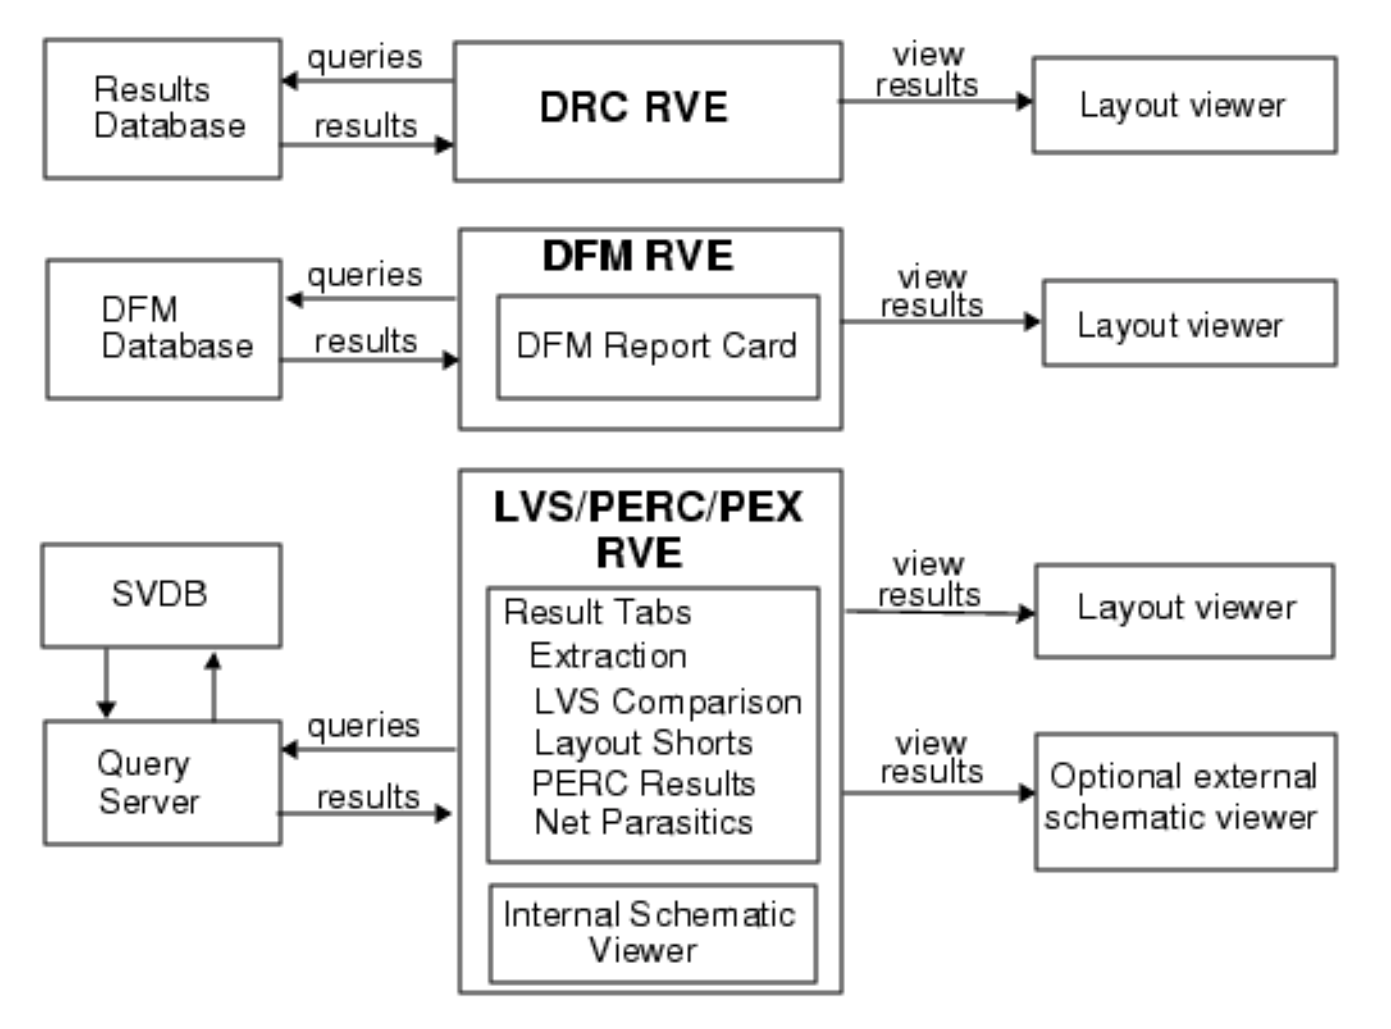
\includegraphics[scale=0.125]{Fig/lvs2.png} 
\vspace{-0.1in}
\caption{Output from RVE.}
\end{figure}
\end{center}
\end{frame}
%%%%%%%%%%%%%%%%%%%%%%%%%%%%%%%%%%%%%%%%%%%%%%%%%%%%%%%%%%%%%%%%%%%%
\begin{frame}
\frametitle{LVS Typical Flow}
\begin{center}
\begin{figure}
	\vspace{-0.1in}
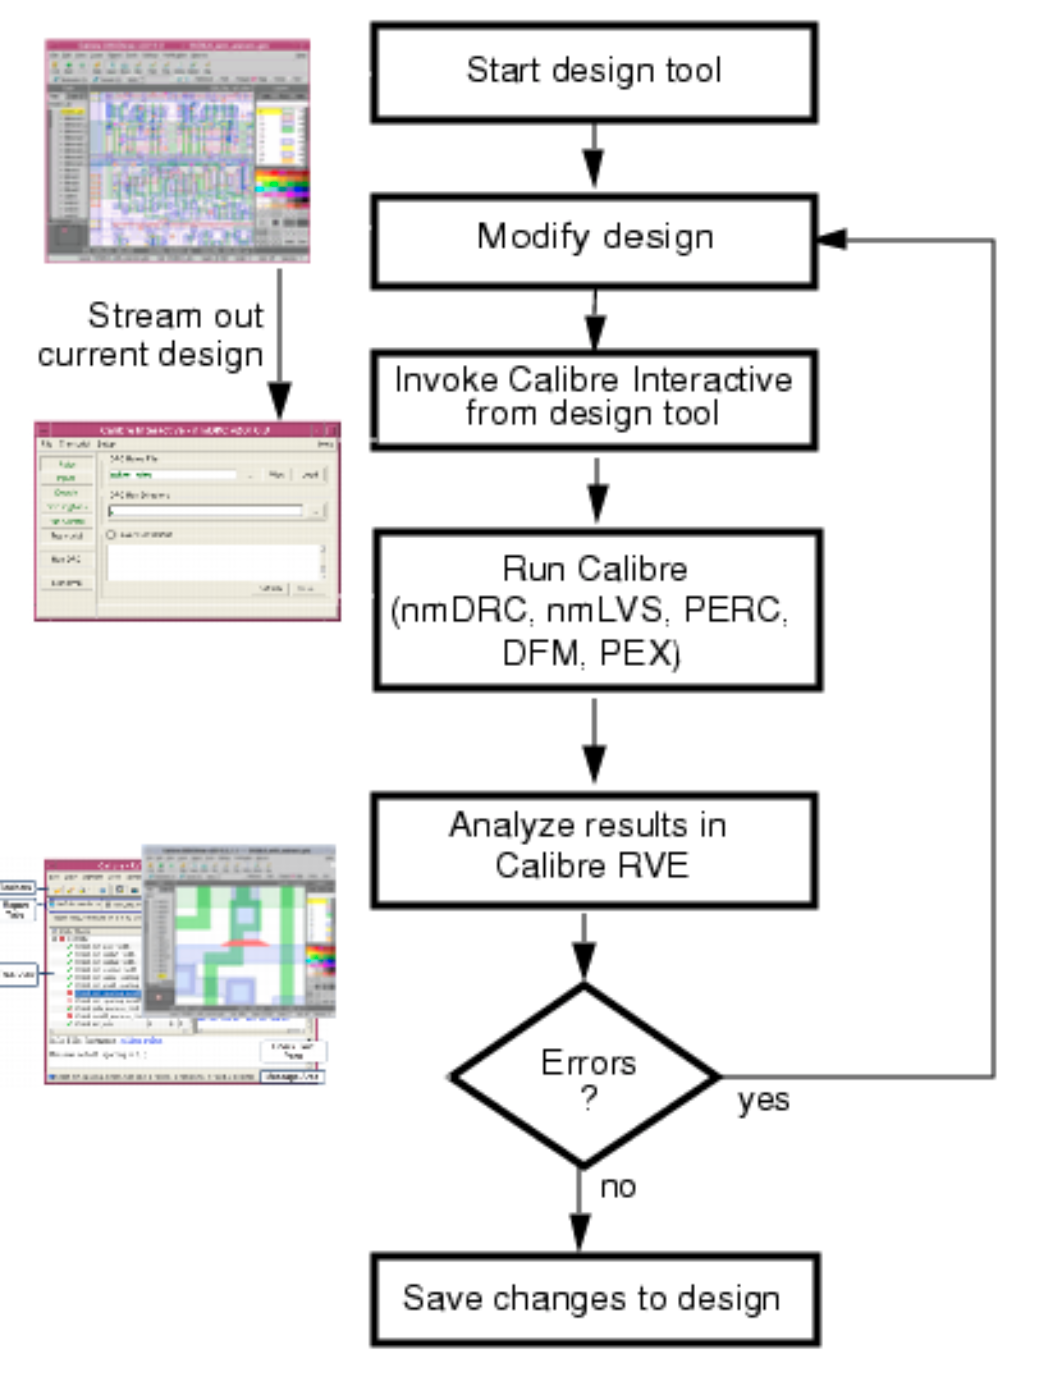
\includegraphics[scale=0.125]{Fig/lvs1.png} 
\vspace{-0.1in}
\caption{Typical LVS Flow using Mentor Graphics Calibre.}
\end{figure}
\end{center}
\end{frame}
%%%%%%%%%%%%%%%%%%%%%%%%%%%%%%%%%%%%%%%%%%%%%%%%%%%%%%%%%%%%%%%%%%%%
\begin{frame}[fragile]
\frametitle{Batch Basis}
\begin{itemize}
\item RVE is great, but it takes time to run.  Therefore, its
  convenient to run LVS batch based.
\item Calibre runs things batch based through something called
  Runsets.
\item A \textit{Runset} is a Calibre-Interactive-generated file that stores the
  settings you specify in the GUI windows
\item Runset files are typically ASCII files in your current working
  directory - they are typically called \verb+.runset.calibre.lvs+
  where the last item is typically the Calibre program it utilizes. 
\end{itemize}
\end{frame}
%%%%%%%%%%%%%%%%%%%%%%%%%%%%%%%%%%%%%%%%%%%%%%%%%%%%%%%%%%%%%%%%%%%%
\begin{frame}[fragile]
\frametitle{Preliminaries}
\begin{itemize}
\item Before one starts a LVS, a layout is required to check against a
  netlist.  Most often this is the layout generated from a System on
  Chip place and route and usually will come with a gds and Verilog
  netlists.
\item To start bringing in the layout to get ready for LVS, a simple
  SKILL file was created to create a blank layout.  This script can be
  run with the following 
  command: \verb+virtuoso -nograph -replay CreateLib.il -log CreateLib.log+
\item The SKILL script is as follows creating a library for
  \verb+tcore+ (i.e., any name can be given) and binds it to the
  GF 32nm design library and its associated rules.
\end{itemize}
\footnotesize
\begin{verbatim}
(setq libName "tcore");
(setq techFile "cmos32soi");
(ddCreateLib libName);
(setq libId (ddGetObj libName));
(techBindTechFile libId techFile);
\end{verbatim}
\normalsize
\end{frame}
%%%%%%%%%%%%%%%%%%%%%%%%%%%%%%%%%%%%%%%%%%%%%%%%%%%%%%%%%%%%%%%%%%%%
\begin{frame}[fragile]
\frametitle{strmin}
\begin{itemize}
\item Once the library has been created, your gds layout can be
  brought in to make sure its ready for LVS.
\item This can be done with the \verb+strmin+ Cadence Design Systems (CDS)
  command.  The \verb+strmin+ command is an updated command that
  replaces the Pipe-In-Pipe-Out or PIPO command.
\item To run \verb+strmin+ a template file is needed (as shown on the
  next slide).
  \begin{itemize}
  \item The command to run is \verb+strmin -templateFile streamOut.templatefile+
  \end{itemize}
\item Once the layout is brought in a label needs to be created
  anywhere on the layout to designate the substrate layer with the
  name \verb+soisub!+.
\end{itemize}
\end{frame}
%%%%%%%%%%%%%%%%%%%%%%%%%%%%%%%%%%%%%%%%%%%%%%%%%%%%%%%%%%%%%%%%%%%%
\begin{frame}[fragile]
\frametitle{streamIn.template}
\footnotesize
\begin{verbatim}
runDir                          "."
library                         "tcore"
strmFile                        "T_CORE_0.calibre.db"
topCell                         "T_CORE_0" 
view                            "layout"
refLibList                      "refLib.list"
snapToGrid                      "true"
runDir                          "."
case                            "preserve"
writeMode                       "overwrite"
checkPolygon                    "t"
logFile                         "strmIn.log"
summaryFile                     "strmIn_summary.log"
\end{verbatim}
\normalsize
\end{frame}
%%%%%%%%%%%%%%%%%%%%%%%%%%%%%%%%%%%%%%%%%%%%%%%%%%%%%%%%%%%%%%%%%%%%
\begin{frame}[fragile]
\frametitle{Running Calibre LVS}
\begin{itemize}
\item Any Calibre tool must be set up properly, therefore, a proper
  \verb+.cshrc+ file should be utilized to set the path properly.
\item To run the Interactive Calibre LVS, you can type the following:
  \verb+calibre -gui -lvs+.
\item To run Calibre LVS as a batch item, type: 
\tiny
\begin{verbatim}
calibre -gui -app -runset_options_display my_runset -batch >& batch.log
\end{verbatim}
\normalsize
where \verb+my_runset+ is your Runset for your LVS run and \verb+app+
is \verb+-lvs+.
\item Output is typically stored in log files (e.g.,
  layoutLibrary.lvs.report) and graphics output is stored in the
  \verb+svdb+ directory.
\item You can call up the graphical output by typing \verb+calibrerve+.
\end{itemize}
\end{frame}
%%%%%%%%%%%%%%%%%%%%%%%%%%%%%%%%%%%%%%%%%%%%%%%%%%%%%%%%%%%%%%%%%%%%
\begin{frame}[fragile]
\frametitle{Precursor Files}
\begin{itemize}
\item Calibre needs some files to get started, which include:
\begin{itemize}
\item Source gds that you want to compare
\item Source netlist (usually as a Verilog file)
\end{itemize}
\item The source gds is important and to make things easier, its
  convenient to export your layout as a batch-based process, as well.
\item Early CDS layouts utilized PIPO or Pipe-In,
  Pipe-Out, but this has changed to a utility called \verb+strmin+ and
  \verb+strmout+ for exporting and importing, respectively.
\item This is streamlined utilizing a \verb+templateFile+ to set the
  export capabilities.
\begin{itemize}
\item The command to run is \verb+strmout -templateFile streamOut.templatefile+
\end{itemize}
\end{itemize}
\end{frame}
%%%%%%%%%%%%%%%%%%%%%%%%%%%%%%%%%%%%%%%%%%%%%%%%%%%%%%%%%%%%%%%%%%%%
\begin{frame}[fragile]
\frametitle{streamOut.template}
\footnotesize
\begin{verbatim}
runDir                          "."
library                         "tcore"
strmFile                        "T_CORE_0.calibre.db"
topCell                         "T_CORE_0" 
view                            "layout"
snapToGrid                      "true"
runDir                          "."
case                            "preserve"
checkPolygon                    "t"
logFile                         "strmOut.log"
summaryFile                     "strmOut_summary.log"
convertDot                      "node"
hierDepth                       "32767"
\end{verbatim}
\normalsize
\end{frame}
%%%%%%%%%%%%%%%%%%%%%%%%%%%%%%%%%%%%%%%%%%%%%%%%%%%%%%%%%%%%%%%%%%%%
\begin{frame}[fragile]
\frametitle{strmOut oddities}
\begin{itemize}
\item There are some items to be aware of with strmout, which is
  called XStream Out inside CDS tools.
\item Any gds output should include the standard-cells, so you need to
  \textbf{leave off} any reference to libraries, which is usually indicated by 
  \verb+refLibList+ in the \verb+strmin+ templateFile.
\item Calibre usually calles its gds that it imports a .db file
  although it is technically a gds file.
\item Although not needed, \verb+snapToGrid+ is utilized to avoid any
  problems with roundoff of any floating-point number.
\item To avoid any problems with hiearchy, the \verb+hierDepth+ is set
  to its maximum value of $32767$.
\end{itemize}
\end{frame}
%%%%%%%%%%%%%%%%%%%%%%%%%%%%%%%%%%%%%%%%%%%%%%%%%%%%%%%%%%%%%%%%%%%%
\begin{frame}[fragile]
\frametitle{Calibre Batch}
\begin{itemize}
\item To run Calibre in batch, a runset is utilized.
\item Any output will be in the \verb+file.lvs.report+ file dictated
  by what is defined in the \verb+Runset+.
\item Although you can change the output directory where the results
  go for the \verb+calibrerve+, it does not seem to work efficiently
  (despite options in the Runset to change this directory name).
  Therefore, it is advisable just to store it in the \verb+svdb+
  directory and move the directory manually, if needed, for now.
\item The Verilog netlist must be translated into an equivalent SPICE
  deck.  This is accomplished using the following command:
\begin{verbatim}
v2lvs -v file.v -o _file.v.sp -w 2
\end{verbatim}
\item The default SPICE deck needed for Calibre LVS requires that the output
  from \verb+v2lvs+ have an underscore as a prefix
\end{itemize}
\end{frame}
%%%%%%%%%%%%%%%%%%%%%%%%%%%%%%%%%%%%%%%%%%%%%%%%%%%%%%%%%%%%%%%%%%%%
\begin{frame}[fragile]
\frametitle{Results Viewing Environment (RVE)}
\begin{itemize}
\item Errors or any output can be easily read through the LVS report,
  however, its nice to have a method to read output graphically.  This
  is provided by Calibrerve or Results Viewing Environment (RVE).
\item To invoke, just type \verb+calibrve+
\item You can easily load any results through the directory created by
  LVS that is typically called svdb or the Mask SVDB directory.
\item This directory typically writes Standard Verification Results
  File information that is standard across Calibre tools.
\item RVE can be utilized to identify errors and hopefully fix them.
\end{itemize}
\end{frame}
%%%%%%%%%%%%%%%%%%%%%%%%%%%%%%%%%%%%%%%%%%%%%%%%%%%%%%%%%%%%%%%%%%%%
\begin{frame}
\frametitle{RVE Screen}
\begin{center}
\begin{figure}
	\vspace{-0.1in}
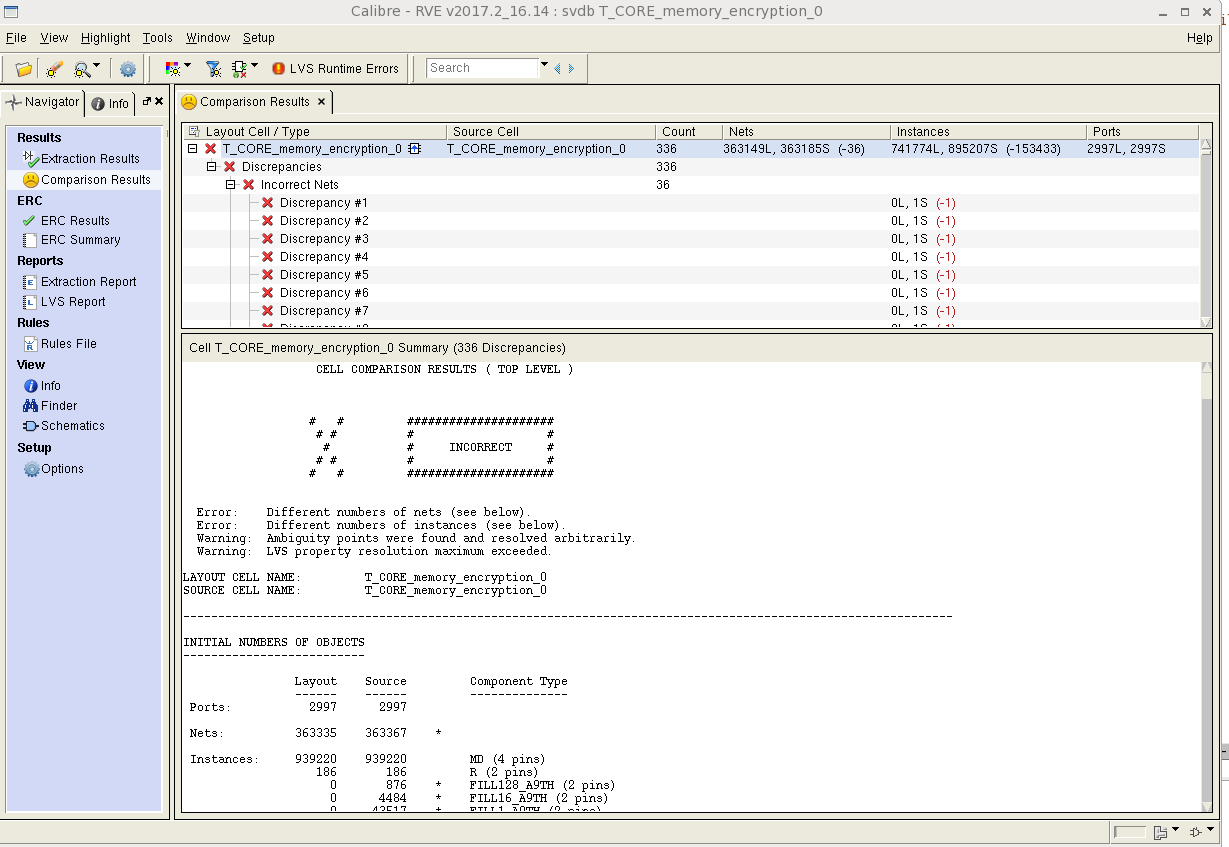
\includegraphics[scale=0.23]{Fig/lvs2-2.png} 
\vspace{-0.1in}
\caption{Calibre RVE Output showing Errors.}
\end{figure}
\end{center}
\end{frame}
%%%%%%%%%%%%%%%%%%%%%%%%%%%%%%%%%%%%%%%%%%%%%%%%%%%%%%%%%%%%%%%%%%%%
\begin{frame}[fragile]
\frametitle{RVE Graphical Interaction}
\begin{itemize}
\item SVDB directories can be loaded within RVE.
\item However, sometimes its nice to have some sort of idea what the
  problems are. 
\item Although RVE has netlist information, it does not always have
  information about the layout.
\item Fortunately, Mentor Graphics have created a new tool called
  Calibre DESIGNrev.
\begin{itemize}
\item Calibre DESIGNrev is a layout tool that allows you to pull up
  layout more efficiently than through CDS's layout
  editor Virtuoso.
\item The important part about Calibre DESIGNrev is that it has
  graphical information feedback through RVE (although CDS Virtuoso has
  this too, but this method is faster).
\item Calibre recommends this tool in their flow for checking and
  debugging errors as shown on the next slide.
\item To run Calibre DESIGNrev, type \verb+calibredrv+.
\end{itemize}
\end{itemize}
\end{frame}
%%%%%%%%%%%%%%%%%%%%%%%%%%%%%%%%%%%%%%%%%%%%%%%%%%%%%%%%%%%%%%%%%%%%
\begin{frame}
\frametitle{RVE Methodology}
\begin{center}
\begin{figure}
	\vspace{-0.1in}
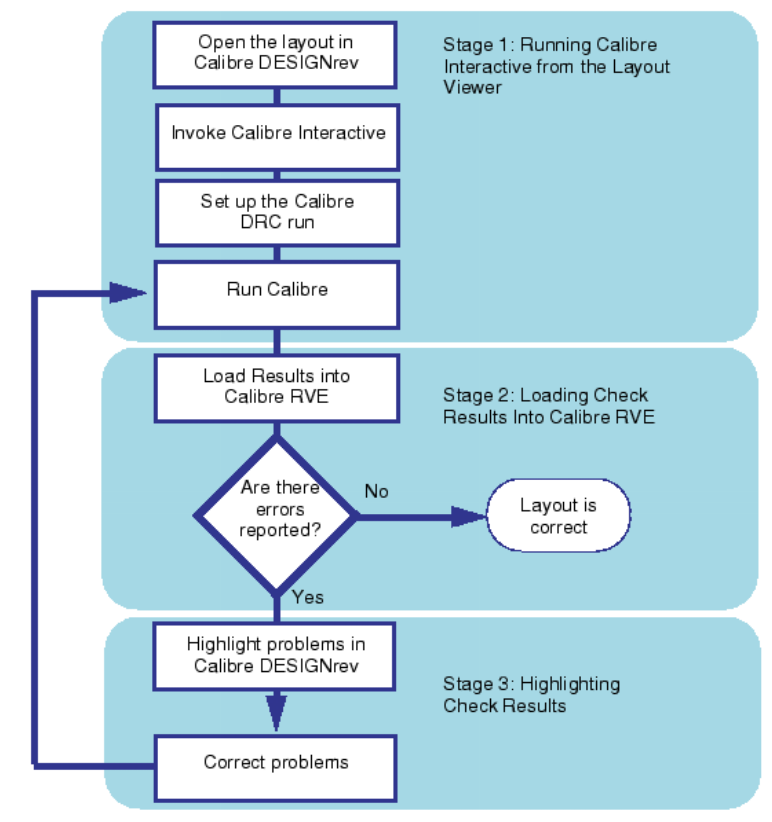
\includegraphics[scale=0.23]{Fig/lvs2-1.png} 
\vspace{-0.1in}
\caption{Calibre RVE FLow.}
\end{figure}
\end{center}
\end{frame}
%%%%%%%%%%%%%%%%%%%%%%%%%%%%%%%%%%%%%%%%%%%%%%%%%%%%%%%%%%%%%%%%%%%%
\begin{frame}
\frametitle{Calibre DESIGNrev Screen}
\begin{center}
\begin{figure}
	\vspace{-0.1in}
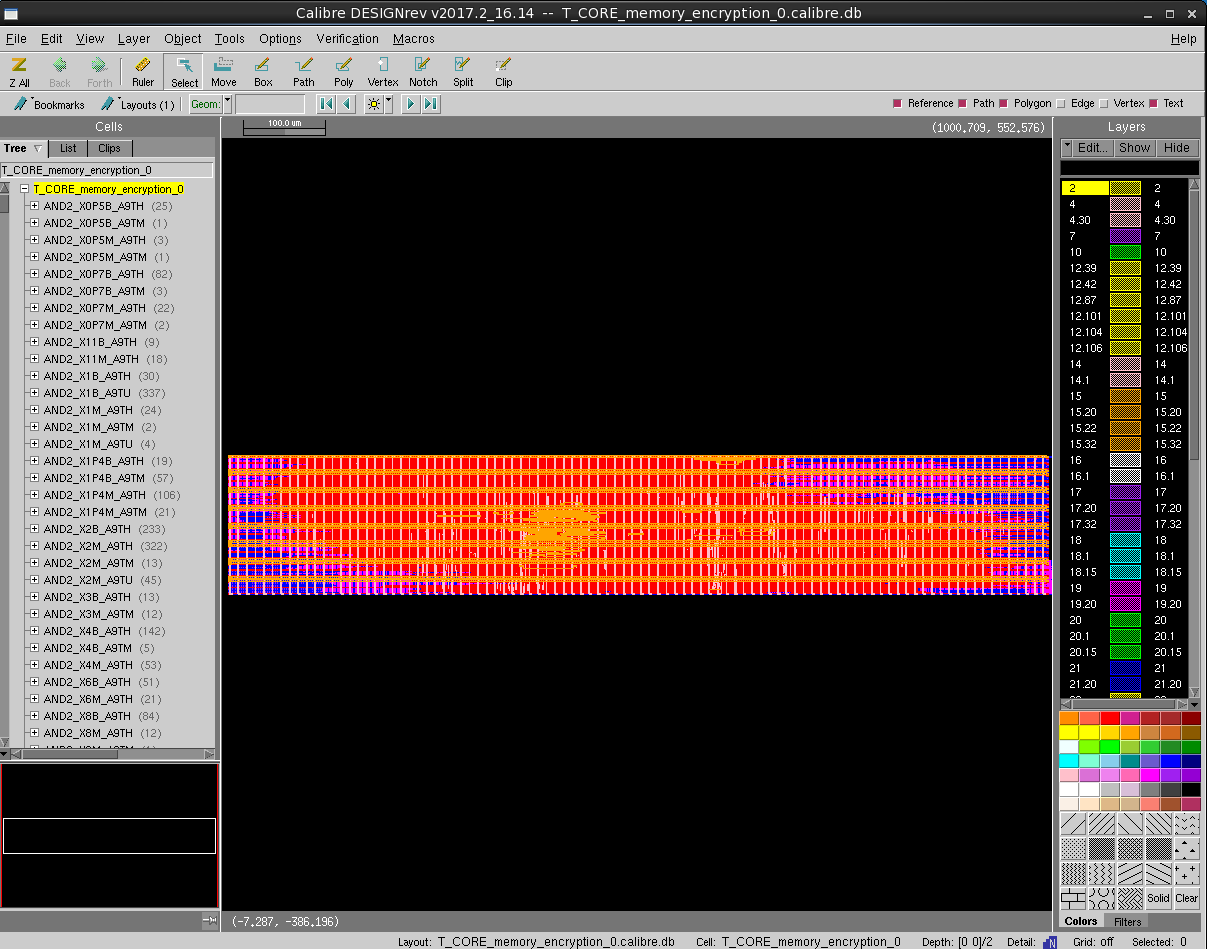
\includegraphics[scale=0.2]{Fig/lvs2-5.png} 
\vspace{-0.1in}
\caption{Calibre DESIGNrev Example Screen.}
\end{figure}
\end{center}
\end{frame}
%%%%%%%%%%%%%%%%%%%%%%%%%%%%%%%%%%%%%%%%%%%%%%%%%%%%%%%%%%%%%%%%%%%%
\begin{frame}[fragile]
\frametitle{Calibre DESIGNrev RVE integration}
\begin{itemize}
\item To run, RVE, first pull up the layout in Calibre DESIGNrev.
\item Under the Verification menu in Calibre DESIGNrev, click RVE
  (interestingly, you can also run any of the Calibre tools from this
  menu, as well).
\item Once RVE is invoked, it will either ask you to enter the
  svdb directory or it might fill it in for you depending on what
  information it can extract from the directory.
\item Once loaded, any error can be pulled up visually to see any
  errors.
\item To document the problem, a VDD-VSS short is shown in the
  following slide.
\end{itemize}
\end{frame}
%%%%%%%%%%%%%%%%%%%%%%%%%%%%%%%%%%%%%%%%%%%%%%%%%%%%%%%%%%%%%%%%%%%%
\begin{frame}
\frametitle{Calibre RVE Error}
\begin{center}
\begin{figure}
	\vspace{-0.1in}
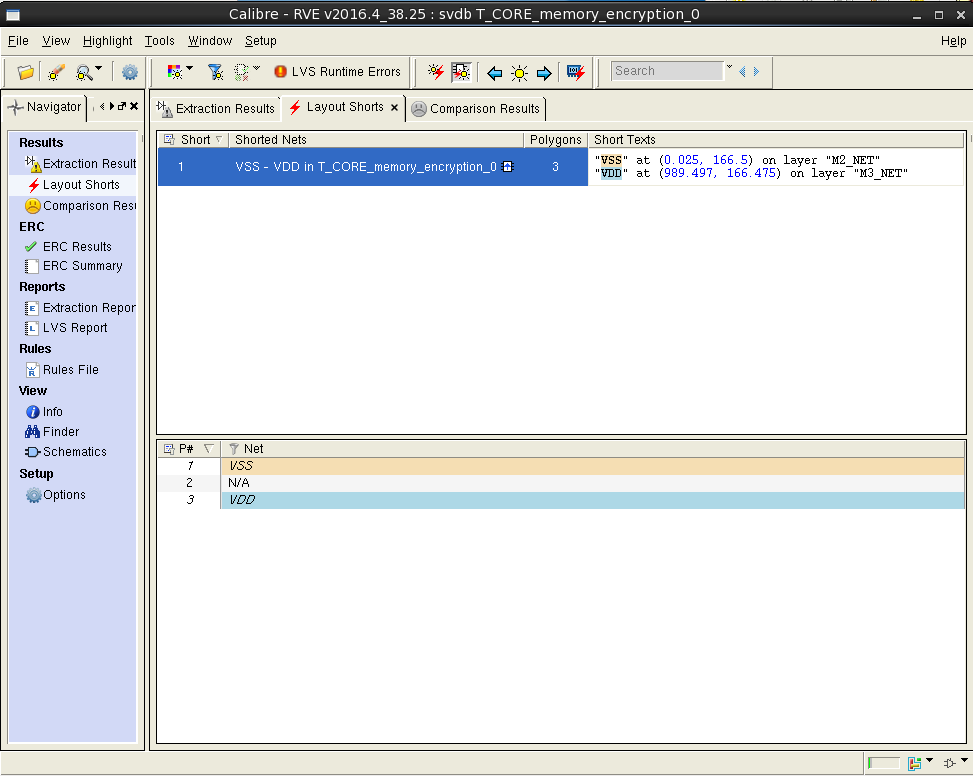
\includegraphics[scale=0.2]{Fig/lvs2-4.png} 
\vspace{-0.1in}
\caption{Calibre DESIGNrev Error showing VDD-VSS Short.}
\end{figure}
\end{center}
\end{frame}
%%%%%%%%%%%%%%%%%%%%%%%%%%%%%%%%%%%%%%%%%%%%%%%%%%%%%%%%%%%%%%%%%%%%
\begin{frame}
\frametitle{Calibre DESIGNrev Screen}
\begin{center}
\begin{figure}
	\vspace{-0.1in}
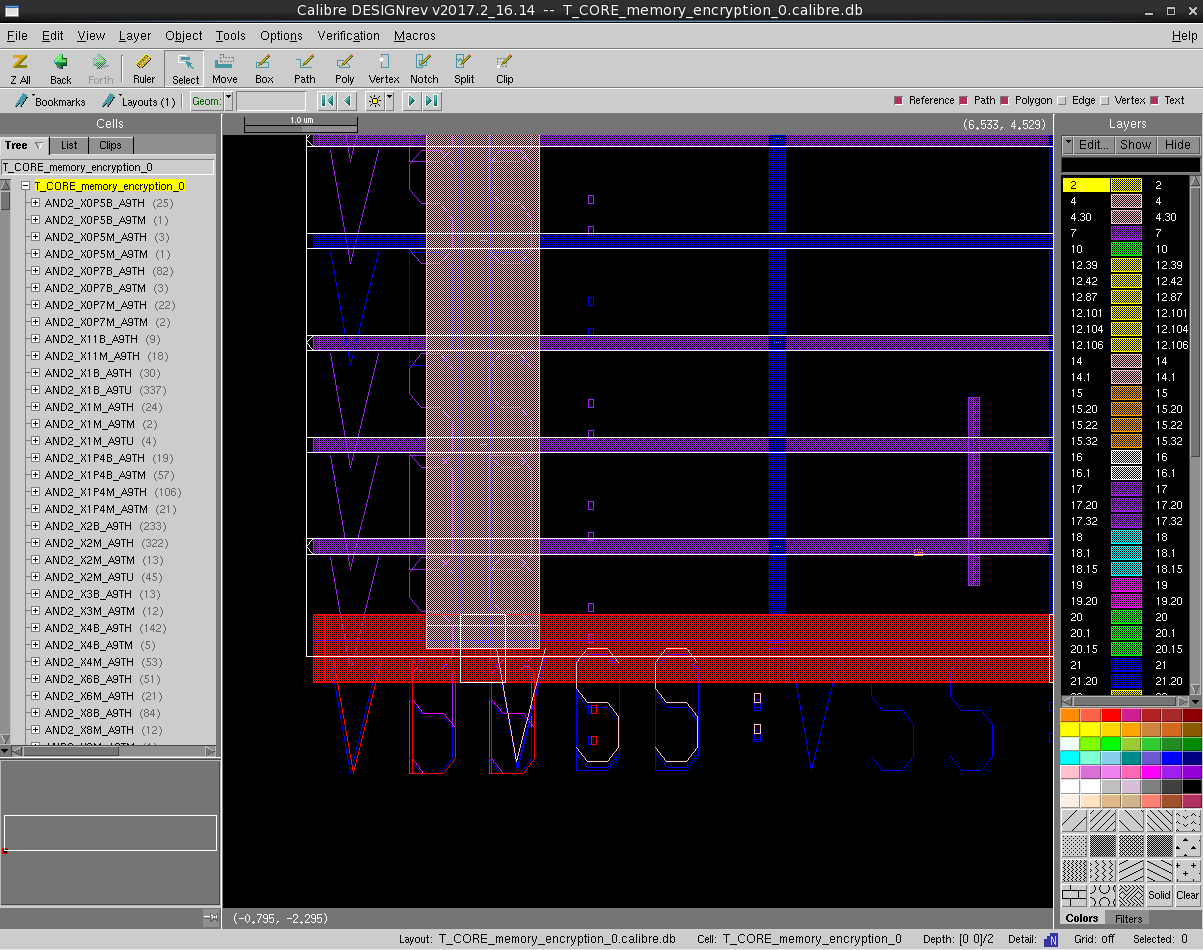
\includegraphics[scale=0.2]{Fig/lvs2-6.png} 
\vspace{-0.1in}
\caption{Clicking RVE screen invokes Calibre DESIGNrev to show error.}
\end{figure}
\end{center}
\end{frame}
%%%%%%%%%%%%%%%%%%%%%%%%%%%%%%%%%%%%%%%%%%%%%%%%%%%%%%%%%%%%%%%%%%%%
\begin{frame}[fragile]
\frametitle{Methodology}
\begin{itemize}
\item The following are the procedure for running the LVS
\begin{enumerate}
\item Locate the gds and netlist you want to compare.  This will
  usually come from CDS' Innovus.
\item First import for checking\footnote{Make sure \textit{soisub!}
  label is present on layout using SXCUT GDS number 62:10},
  \verb+strmin -templateFile streamIn.template+

\end{enumerate}
\end{itemize}
\end{frame}
%%%%%%%%%%%%%%%%%%%%%%%%%%%%%%%%%%%%%%%%%%%%%%%%%%%%%%%%%%%%%%%%%%%%
\begin{frame}[fragile]
\frametitle{Summary}
\begin{itemize}
\item A repeatable batch-based LVS design flow has been introduced.
\item Many Mentor Graphics Calibre tools are utilized to help figure
  out any errors with layout.
\item Other helpful scripts to read in and out gds files as well as
  other small scripts have been introduced.
\item All scripts and this presentation are 
  at \verb+/import/vlsi4/IBM_PDK/cmos32soi/LVS_Stream+
\item Any feedback is welcome to this process.
\end{itemize}
\end{frame}
%%%%%%%%%%%%%%%%%%%%%%%%%%%%%%%%%%%%%%%%%%%%%%%%%%%%%%%%%%%%%%%%%%%%



\end{document}
